% THIS IS SIGPROC-SP.TEX - VERSION 3.1
% WORKS WITH V3.2SP OF ACM_PROC_ARTICLE-SP.CLS
% APRIL 2009
%
% Questions regarding SIGS should be sent to
% Adrienne Griscti ---> griscti@acm.org
%
% Questions/suggestions regarding the guidelines, .tex and .cls files, etc. to
% Gerald Murray ---> murray@hq.acm.org
%
% For tracking purposes - this is V3.1SP - APRIL 2009
%
% Copied from https://github.com/heathermiller/papers-documents/tree/master/rem2013

\documentclass{support/acm_proc_article-sp}
\usepackage{listings}
\usepackage{url}
\usepackage{support/bcprules}
\usepackage{support/prooftree}
\usepackage{support/math}
\usepackage{multicol}
\usepackage{caption}
\usepackage{subcaption}
\usepackage[normalem]{ulem}
\usepackage{color}
\usepackage{graphicx}
\usepackage{hyperref}

\renewcommand{\thesubsection}{\thesection.\alph{subsection}}

\definecolor{blue}{rgb}{0,0,0.5}
\definecolor{red}{rgb}{0.6,0,0}
\definecolor{green}{rgb}{0,0.5,0}
\definecolor{grey}{rgb}{0.2,0.2,0.2}

\lstdefinelanguage{Python}{
keywords={typeof, null, catch, switch, in, int, str, float, self},
keywordstyle=\color{blue}\bfseries,
ndkeywords={boolean, throw, import},
ndkeywords={return, class, if ,elif, endif, while, do, else, True, False , catch, def},
ndkeywordstyle=\color{blue}\bfseries,
identifierstyle=\color{red},
sensitive=false,
comment=[l]{\#},
morecomment=[s]{/*}{*/},
commentstyle=\color{green}\ttfamily,
stringstyle=\color{green}\ttfamily,
}

\lstset{language=Python}

% comments and notes
\newcommand{\comment}[1]{}
\newcommand{\note}[1]{{\bf $\clubsuit$ #1 $\spadesuit$}}
\newcommand{\ifreport}[1]{#1}
%\newcommand{\ifreport}[1]{}

\newcommand{\todo}{{\bf \colorbox{red}{\color{white}TODO:}}}
\newcommand{\ie}{{\em i.e.,~}}
\newcommand{\eg}{{\em e.g.,~}}
\newcommand{\term}[1]{\mbox{\texttt{#1}}}
\newcommand{\itl}[1]{\mbox{\textit{#1}}}

% commas and semicolons
\newcommand{\comma}{,\,}
\newcommand{\commadots}{\comma \ldots \comma}
\newcommand{\semi}{;\mbox{;};}
\newcommand{\semidots}{\semi \ldots \semi}

% spacing
\newcommand{\gap}{\quad\quad}
\newcommand{\biggap}{\quad\quad\quad}
\newcommand{\nextline}{\\ \\}
\newcommand{\htabwidth}{0.5cm}
\newcommand{\tabwidth}{1cm}
\newcommand{\htab}{\hspace{\htabwidth}}
\newcommand{\tab}{\hspace{\tabwidth}}
\newcommand{\linesep}{\ \hrulefill \ \smallskip}

\newcommand{\sectionline}{%
\nointerlineskip \vspace{\baselineskip}%
\hspace{\fill}\rule{0.5\linewidth}{.7pt}\hspace{\fill}%
\par\nointerlineskip \vspace{\baselineskip}
}

% figures
\newcommand{\figurebox}[1]
{\fbox{\begin{minipage}{\textwidth}
           #1 \medskip
\end{minipage}}}
\newcommand{\twofig}[3]
{\begin{figure*}[t]
     #3\ \hrulefill\
        \caption{\label{#1}#2}
\end{figure*}}
\newcommand{\boxfig}[3]
{\begin{figure*}
     \figurebox{#3\caption{\label{#1}#2}}
\end{figure*}}
\newcommand{\figref}[1]
{Figure~\ref{#1}}

% arrays
\newcommand{\ba}{\begin{array}}
\newcommand{\ea}{\end{array}}
\newcommand{\bda}{\[\ba}
\newcommand{\eda}{\ea\]}
\newcommand{\ei}{\end{array}}
\newcommand{\bcases}{\left\{\begin{array}{ll}}
\newcommand{\ecases}{\end{array}\right.}

\pagenumbering{arabic}
\begin{document}

    \title{Hot Topics in Machine Learning (HWS17) \\ Assignment 1: Logistic Regression}

    \numberofauthors{1}
    \author{
    \alignauthor
    Steffen Schmitz\\
    \affaddr{University of Mannheim}\\
    \affaddr{stefschm@mail.uni-mannheim.de}
    }

    \maketitle

    %%%%%%%%%%%%%%%%%%%%%%%%%%%%%%%%%%%%%%%%%%%%%%%%%%%%
    %%
    %% 1) DATASET STATISTICS
    %%
    %%%%%%%%%%%%%%%%%%%%%%%%%%%%%%%%%%%%%%%%%%%%%%%%%%%%

    \section{Dataset Statistics}
    \vspace{1.5\baselineskip}

    Explore and preprocess the dataset.

    %%%%%%%%%%%%%%%%%%%%%%%%%%%%%%%%%%%%%%%%%%%%%%%%%%%%
    %%
    %% 1.a) KERNEL DENSITY PLOT
    %%
    %%%%%%%%%%%%%%%%%%%%%%%%%%%%%%%%%%%%%%%%%%%%%%%%%%%%

    \subsection{Kernel Density Plot}
    \label{sec:kdp}
    \vspace{\baselineskip}

    \textbf{Task.} Look at the kernel density plot (code provided) of all features and discuss what you see (or don't see).

    We estimate the kernel density estimation with the gaussian\_kde method from the scipy.stats
    package\footnote{\href{https://docs.scipy.org/doc/scipy/reference/generated/scipy.stats.gaussian_kde.html}{https://docs.scipy.org/gaussian\_kde}}.
    It returns the estimated probability density function of each feature.
    As described in the documentation the plot may be "oversmoothed" what leads to non-zero results for $x < 0$,
    although the statistics (Output of Figure \ref{fig:describe}) show that all features have minimal values that are
    greater or equal to zero.

    \begin{figure}[!htbp]
        \centering
        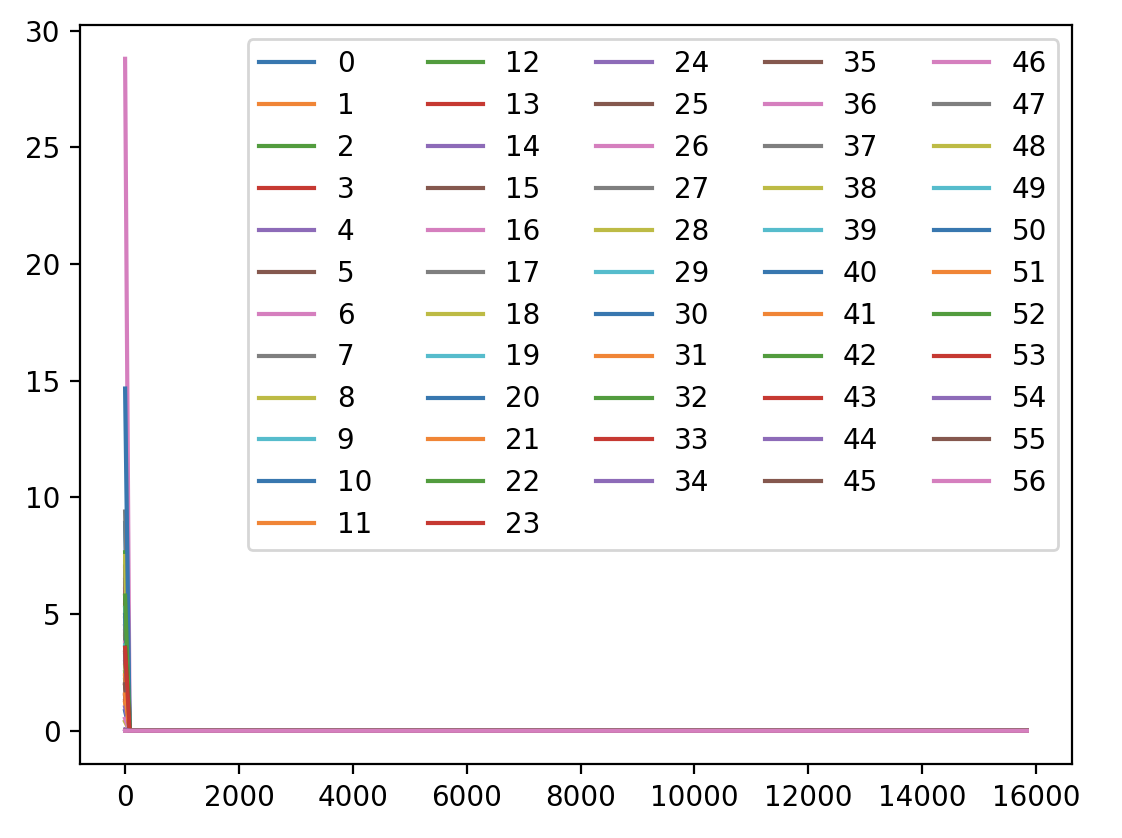
\includegraphics[width=8cm]{images/kdp.png}
        \caption{Unregularized Kernel Density Plot}
        \label{fig:kernel-density-plot}
    \end{figure}

    Figure \ref{fig:kernel-density-plot} displays the result of the gaussian\_kde for the training dataset.
    The x-axis has a scale from 0 to 16000 and the y-axis ranges from 0 to 30.
    We can see that almost all data is close to zero and all features approximate zero asymptotically for values $x >> 0$.

    There are four visible spikes at $x \approx 0$ that range to about 28, 15, 10 and 4, respectively.
    All other features are either smaller or overwritten by the latest features.

    The behaviour that is observed in the graph is confirmed by the dataset's statistics that we get by executing the
    code in Figure \ref{fig:describe}.
    \begin{figure}[htbp]
        \centering
        \lstset{numbers=none,xleftmargin=0em}
        \lstinputlisting{listings/describe.py}
        \caption{Show statistics about the data.}
        \label{fig:describe}
    \end{figure}
    The features 0 to 54 are percentages and, therefore, have a range from 0 to 1, while the other features are counts of
    uppercase letters in the e-mail.
    Their minimum is 1 and the maximum can range into the thousands.

    From this we can subsume that the current visualization is insufficient, because a few features that can take large numbers
    overshadow the features that represent percentages.
    It is hard to draw any conclusions about the data under the current circumstances.

    %%%%%%%%%%%%%%%%%%%%%%%%%%%%%%%%%%%%%%%%%%%%%%%%%%%%
    %%
    %% 1.b) NORMALIZATION USING Z-SCORES
    %%
    %%%%%%%%%%%%%%%%%%%%%%%%%%%%%%%%%%%%%%%%%%%%%%%%%%%%

    \subsection{Normalization using z-scores}
    \vspace{\baselineskip}

    \textbf{Task.} Normalize the data using z-scores, i.e., normalize each feature to mean 0 and variance 1.
    Normalize both training and test data.
    In particular, think about how test data should be normalized.

    For machine learning algorithms it is often helpful to normalize or scale the features to avoid huge
    coefficients or the dominance of a few features in algorithms, which use the euclidean distance as their error function.
    It also makes gradient descent converge faster compared to the convergence on unnormalized data \cite{DBLP:journals/corr/IoffeS15}.

    The z-score or standard score transforms the features to a normal distribution with mean 0 and variance 1 and is
    computed with:
    \begin{equation}
        z = \frac{x - \mu}{\sigma}
        \label{eq:z-score}
    \end{equation}
    where $\mu$ is the mean and $\sigma$ the standard deviation \cite{standardization}.

    The sklearn.preprocessing package contains a StandardScaler that normalizes features with the z-score
    \footnote{\href{http://scikit-learn.org/stable/modules/generated/sklearn.preprocessing.StandardScaler.html}{http://scikit-learn.org/StandardScaler}}.

    \begin{figure}[htbp]
        \centering
        \lstset{numbers=none,xleftmargin=0em}
        \lstinputlisting{listings/normalization.py}
        \caption{Normalization using sklearn.}
        \label{fig:normalization}
    \end{figure}

    Figure \ref{fig:normalization} shows how to apply the normalization to input array $X$ to get output array $Xz$.
    At first, is fits the mean and standard deviation to $X$ and, secondly, transforms it into a new array.
    This enables the transformation with the same values to the test set to guarantee that the scaled value
    for every input is computed alike in the training and the test set.

    The input arrays $X$ and $Xtest$ are transformed into $Xz$ and $Xtestz$.

    %%%%%%%%%%%%%%%%%%%%%%%%%%%%%%%%%%%%%%%%%%%%%%%%%%%%
    %%
    %% 1.c) NORMALIZED KERNEL DENSITY PLOT
    %%
    %%%%%%%%%%%%%%%%%%%%%%%%%%%%%%%%%%%%%%%%%%%%%%%%%%%%

    \subsection{Normalized Kernel Density Plot}
    \vspace{\baselineskip}

    \textbf{Task.} Redo the kernel density plot on the normalized data.
    What changed?
    Is there anything that "sticks out"?

    Figure \ref{fig:normalized-kernel-density-plot} shows the estimated probability density functions after normalization.
    The x-axis' range is $[-6\sigma, 6\sigma]$ and it includes negative values that are now valid due to the changes
    made on the dataset.
    We use the six sigma range, because it contains almost all datapoints (99,99966\%).
    \begin{figure}[!htbp]
        \centering
        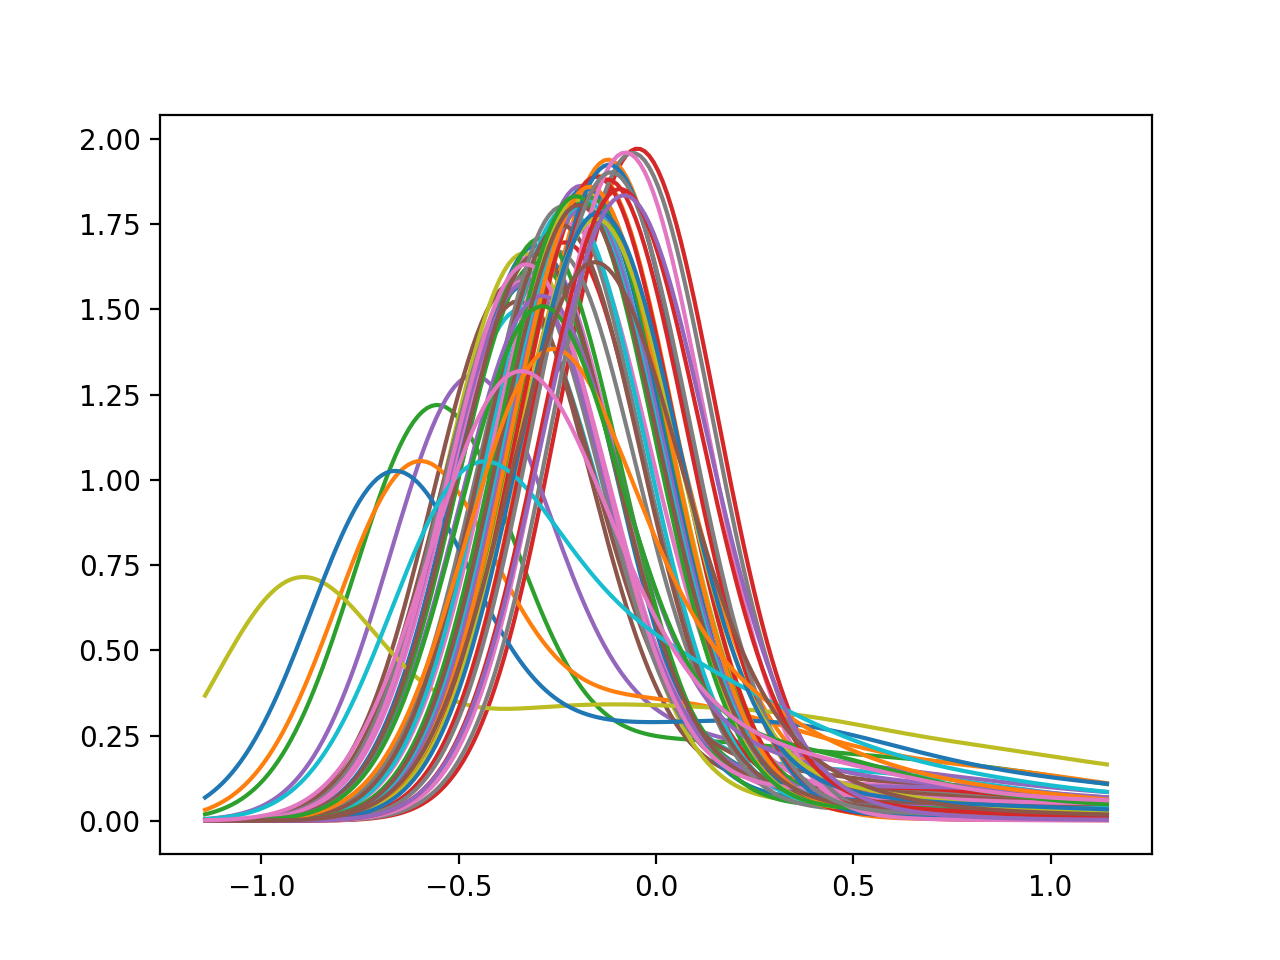
\includegraphics[width=8cm]{images/normalized-kdp.png}
        \caption{Normalized Kernel Density Plot}
        \label{fig:normalized-kernel-density-plot}
    \end{figure}
    After the transformations all features take values in the range $[-1, 46]$ and we can see in Figure \ref{fig:normalized-kernel-density-plot}
    that some features have a positive skew.
    This means that most data points of those features are concentrated on the left side of the graph or around zero, respectively.
    This is supported by the fact that the features have a mean of zero and variation one, but show huge positive values,
    compared to the smallest negative value.
    Those values could be some outliers that may be interesting for the machine learning algorithm.

    The new plot improved the readability and allows to make inferences about the data.
    The data also points to features or values that may become relevant for the algorithm and the training phase.

    %%%%%%%%%%%%%%%%%%%%%%%%%%%%%%%%%%%%%%%%%%%%%%%%%%%%
    %%
    %% 2) MAXIMUM LIKELIHOOD ESTIMATION
    %%
    %%%%%%%%%%%%%%%%%%%%%%%%%%%%%%%%%%%%%%%%%%%%%%%%%%%%

    \section{Maximum Likelihood Estimation}
    \vspace{1.5\baselineskip}

    %%%%%%%%%%%%%%%%%%%%%%%%%%%%%%%%%%%%%%%%%%%%%%%%%%%%
    %%
    %% 2.a) EFFECTS OF RESCALING
    %%
    %%%%%%%%%%%%%%%%%%%%%%%%%%%%%%%%%%%%%%%%%%%%%%%%%%%%

    \subsection{Effects of Rescaling}
    \label{sec:rescaling}
    \vspace{\baselineskip}

    \textbf{Task.} Show analytically that rescaling (multiply by constant) and shifting (add a constant) features leads
    to ML estimates with the same likelihood if there is a bias term.
    Why do you think we computed z-scores then?

    In Maximum Likelihood Estimation (MLE) we try to find a value $\hat{\theta}$ that maximizes the likelihood $\mathcal{L}$
    that we see the values observed in a given sample $\mathbf{X}$\cite[p.316]{CaseBerg:01}.

    Supposing that $\hat{\theta}$ is the MLE of $\theta$, then we want to prove that transforming the input by rescaling and
    shifting leads to an MLE of $f(\hat{\theta})$ for $f(\theta)$, where $f$ is, in our example, the function in equation \ref{eq:z-score}.

    Casella and Berger show in that we get the same answer for the likelihood if the function $f$ is a one-to-one function.
    This is called the "invariance property of maximum likelihood estimators". \cite[p.319]{CaseBerg:01}

    To show that equation \ref{eq:z-score} is one-to-one it suffices to show that $f(x) = f(y) \Rightarrow x = y$ \cite{101978}.
    \begin{equation*}
        f(x) = \frac{x - \mu}{\sigma} = f(y) = \frac{y - \mu}{\sigma} \mbox{  ;    } \cdot \sigma
    \end{equation*}
    \begin{equation*}
        \Leftrightarrow x - \mu = y - \mu \mbox{  ;    } + \mu
    \end{equation*}
    \begin{equation*}
        \Leftrightarrow x = y
    \end{equation*}
    The z-score, therefore, is a one-to-one function and yields the same maximum likelihood estimate.

    Feature scaling or normalization is desirable, because it improves the convergence of gradient descent, without changing
    the accuracy of the predictions \cite{DBLP:journals/corr/IoffeS15}.

    % Skip b, c, d, because they are only about implementation
    \stepcounter{subsection}
    \stepcounter{subsection}
    \stepcounter{subsection}

    %%%%%%%%%%%%%%%%%%%%%%%%%%%%%%%%%%%%%%%%%%%%%%%%%%%%
    %%
    %% 2.e) COMPARE GRADIENT DESCENT WITH STOCHASTIC
    %%      GRADIENT DESCENT
    %%
    %%%%%%%%%%%%%%%%%%%%%%%%%%%%%%%%%%%%%%%%%%%%%%%%%%%%

    \subsection{Compare Gradient Descent with Stochastic Gradient Descent}
    \vspace{\baselineskip}

    \textbf{Task.} Explore the behavior of both methods for the parameters provided to you.
    Discuss!

    The gradient descent converges to a fixed error in about 13 epochs and reduces epsilon to zero after about
    25 epochs.
    The reduction of epsilon needs the same number of epochs in the stochastic gradient descent, but it converges
    faster to the approximate minimum.
    It only needs about 7 epochs.
    The convergence of both algorithms is shown in Figure \ref{fig:gd-vs-sgd}.

    \begin{figure}[!htbp]
        \centering
        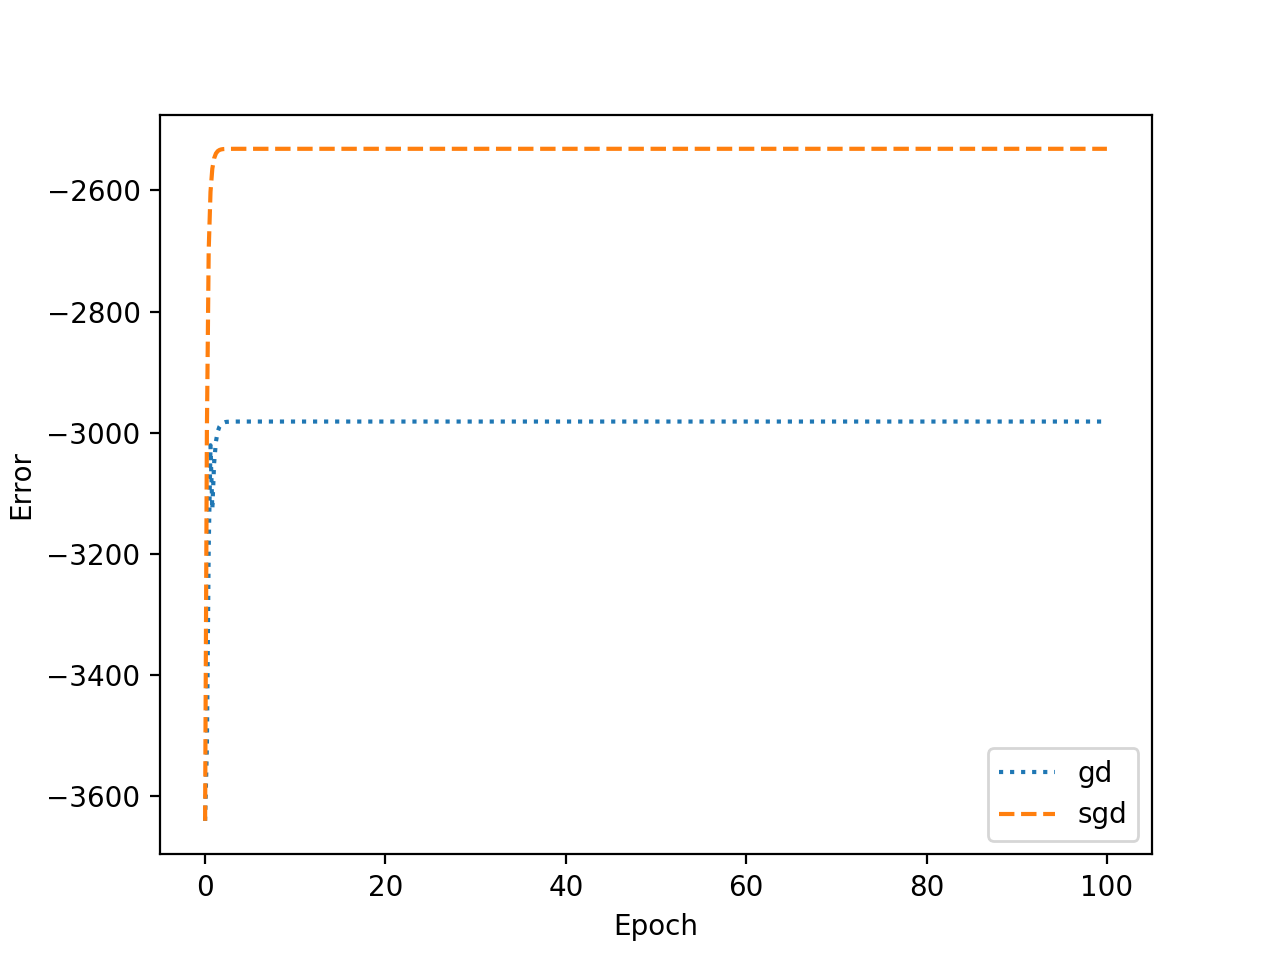
\includegraphics[width=8cm]{images/gd-vs-sgd.png}
        \caption{Gradient Descent vs Stochastic Gradient Descent}
        \label{fig:gd-vs-sgd}
    \end{figure}

    Differences of the algorithms include that the gradient descent is deterministic as it will find the same optimum in
    the same number of steps, while the stochastic gradient descent has some randomness included due to the random
    selection of the samples.
    The number of steps to converge and the exact optimum may, therefore, change between different runs of stochastic gradient
    descent.

    Another feature of stochastic gradient descent is that it reduces the memory footprint.
    While gradient descent computes the updated weights and updates them all at once, the stochastic gradient descent
    does this incrementally.

    As we can see in Figure \ref{fig:gd-vs-sgd} the error computed by stochastic gradient descent is also lower than the
    gradient descent error.
    We would expect them to converge to the same optimum.
    The error might be caused by a numerical trick in the definition of the log-likelihood function, which we use to avoid
    the division by zero.

    %%%%%%%%%%%%%%%%%%%%%%%%%%%%%%%%%%%%%%%%%%%%%%%%%%%%
    %%
    %% 3) PREDICTION
    %%
    %%%%%%%%%%%%%%%%%%%%%%%%%%%%%%%%%%%%%%%%%%%%%%%%%%%%

    \section{Prediction}
    \vspace{\baselineskip}

    \textbf{Task.}
    Complete the predict and classify methods for the predicted spam probability and predicted class label, respectively.
    Explore the models that you fit in the previous task and discuss.
    Study the composition of the weight vector: which features are important, which are not?
    Is this intuitive?

    For gradient descent and stochastic gradient descent we get a parameter vector $wz\_gd$ and $wz\_sgd$, respectively,
    that is fitted to our normalized training set.
    To make predictions we multiply the test set $Xtestz$ with the fitted parameter vectors and compute the sigmoid function
    of the result.
    If the result for a feature is bigger than 0.5 we set it to 1 and 0 for all other results.
    The implementation is shown in Figure \ref{fig:predict-classify}.
    \begin{figure}[htbp]
        \centering
        \lstset{numbers=none,xleftmargin=0em}
        \lstinputlisting{listings/predict-classify.py}
        \caption{Methods to predict and classify the test set.}
        \label{fig:predict-classify}
    \end{figure}
    Using the scikit-learn classification-report\footnote{\href{http://scikit-learn.org/stable/modules/generated/sklearn.metrics.classification_report.html}{http://scikit-learn.org/classification\_report}}
    we get the Precision, Recall and F1-Score for both, stochastic and normal gradient descent.
    The results for gradient descent and stochastic gradient descent are similar with only a 1\% deviation between them.
    See Figure \ref{fig:results} for more details.

    \begin{figure}[!htbp]
        \centering
        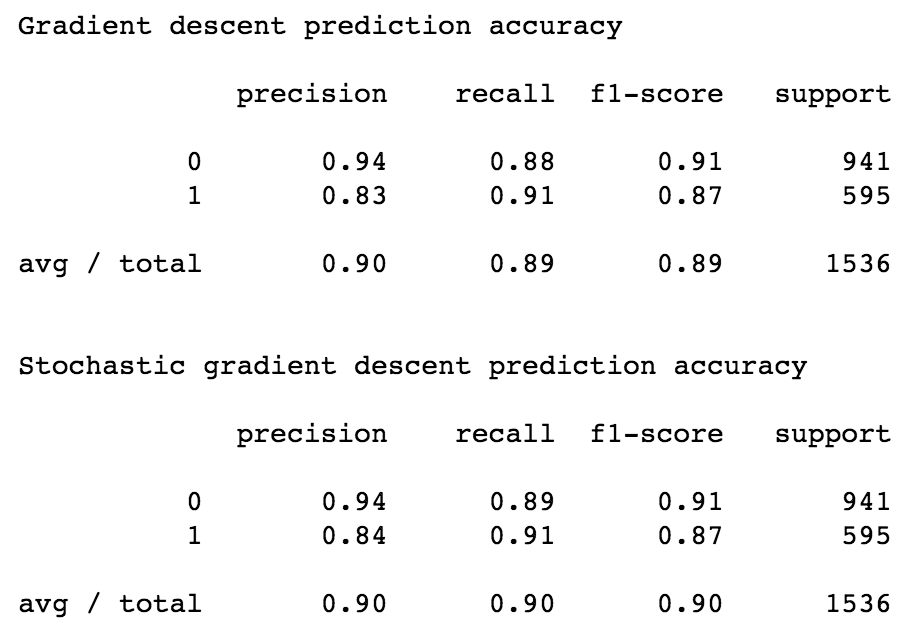
\includegraphics[width=8cm]{images/results.png}
        \caption{Precision, Recall and F1-Score}
        \label{fig:results}
    \end{figure}

    More interesting is that the fitted parameter vectors of gradient descent and stochastic gradient descent differ.
    If we compute the statistics for each parameter vector as described in Figure \ref{fig:describe} we can see that
    the gradient descent has a bigger variance (4.45) in its parameters and has positive skew, while the stochastic
    gradient descent has a variance of 1.52 and a small negative skew (-0.16).

    In the parameter vector of gradient descent there are some features that have a high impact.
    Features 6, 7, 15, 19, 22, 23, 52, 56 have a high positive impact and indicate spam, while features 24, 25 and 41 have
    a big negative impact and, therefore, indicate not-spam.
    They correspond to the frequency of remove, internet, free, credit, 000, money, \$ and the total length of consecutive
    uppercase letters in the case of a positive impact and hp, hpl and meeting in the case of a negative impact.

    As the dataset is provided by the Hewlett-Packard Labs which may be abbreviated as hp or hpl the negative impact of
    those acronyms is not surprising.
    A high frequency of the word meeting is also expected in non-spam e-mails as spammers usually have a low interest in
    meeting their recipients.

    On the other hand, the occurrence of internet, free, credit and money in combination with dollar-signs and many consecutive
    uppercase letters is what we would expect in spam.

    We can draw the conclusion that the weights that are assigned in gradient descent do not come as a surprise and fit
    the common estimate of spam e-mails.

    The parameter vector of stochastic gradient descent shows approximately the same results, but overall, has a smaller variance.
    The outliers are the same, but the overall weights are smaller.

    %%%%%%%%%%%%%%%%%%%%%%%%%%%%%%%%%%%%%%%%%%%%%%%%%%%%
    %%
    %% 4) MAXIMUM APOSTERIORI ESTIMATION
    %%
    %%%%%%%%%%%%%%%%%%%%%%%%%%%%%%%%%%%%%%%%%%%%%%%%%%%%

    \section{Maximum Aposteriori Estimation}
    \vspace{1.5\baselineskip}

    % Skip a, because it is only about implementation
    \stepcounter{subsection}

    %%%%%%%%%%%%%%%%%%%%%%%%%%%%%%%%%%%%%%%%%%%%%%%%%%%%
    %%
    %% 4.b) EFFECT OF PRIOR
    %%
    %%%%%%%%%%%%%%%%%%%%%%%%%%%%%%%%%%%%%%%%%%%%%%%%%%%%

    \subsection{Effect of Prior}
    \label{sec:effect-prior}
    \vspace{\baselineskip}

    \textbf{Task.} Study the effect of the prior on the result by varying the value of $\lambda$.
    Consider at least the training data log-likelihood, the test data log-likelihood, and the prediction accuracy.
    Are these results surprising to you?

    For an initial parameter configuration of $w$, we can see that the log-likelihood takes on huge values for both the
    training and the test data.
    The bigger $\lambda$ is, the bigger is the penalty on large coefficients in the weight vector and the lower the chance
    of overfitting the data.
    An issue may be that the data is underfit for very large values of $\lambda$.

    We can see in the results in Figure \ref{fig:results-lambda} that the F1-Score increases for bigger lambdas, but
    also decreases after a certain threshold.

    \begin{figure}[!htbp]
        \centering
        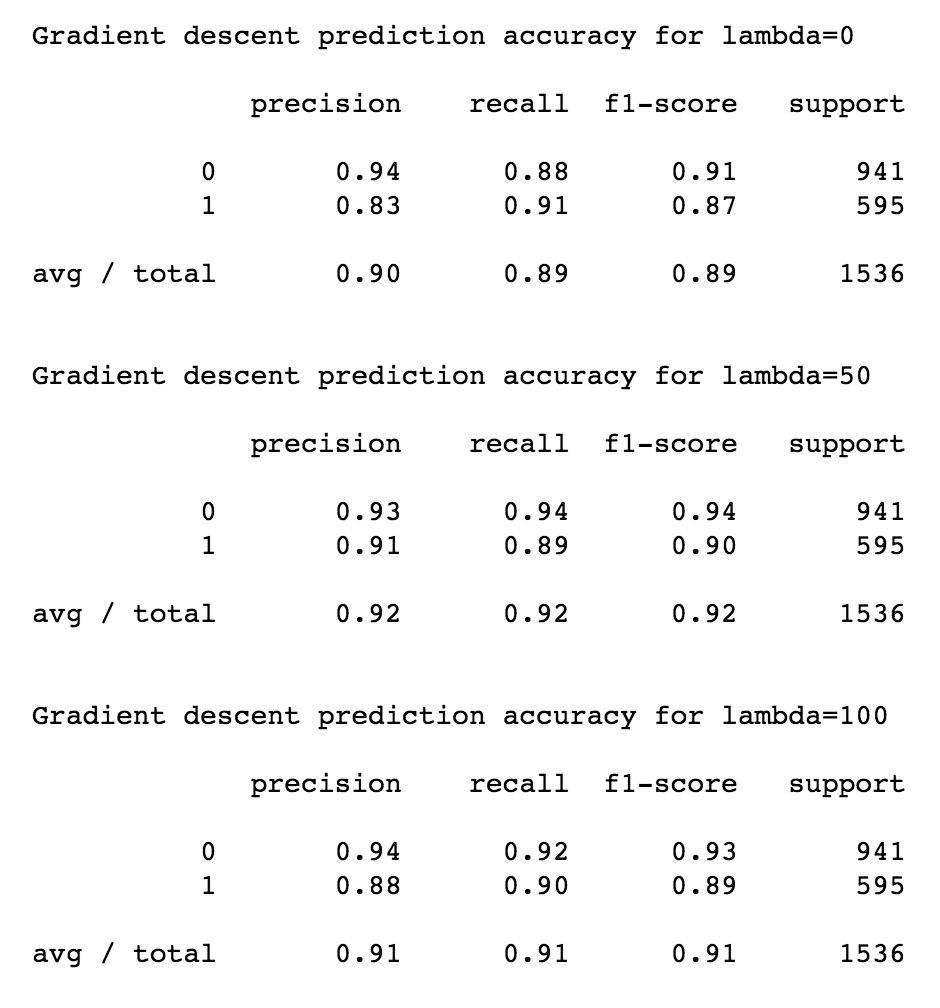
\includegraphics[width=8cm]{images/results-lambda.png}
        \caption{Precision, Recall and F1-Score for different $\lambda$}
        \label{fig:results-lambda}
    \end{figure}

    A way to compute a good value for $\lambda$ would be a cross-validation set that is used to compute different results
    and optimize the F1-Score, by trial-and-error.
    The expected accuracy on unknown data can still be calculated through the test data afterwards.

    %%%%%%%%%%%%%%%%%%%%%%%%%%%%%%%%%%%%%%%%%%%%%%%%%%%%
    %%
    %% 4.c) COMPOSITION OF WEIGHT VECTOR
    %%
    %%%%%%%%%%%%%%%%%%%%%%%%%%%%%%%%%%%%%%%%%%%%%%%%%%%%

    \subsection{Composition of Weight Vector}
    \vspace{\baselineskip}

    \textbf{Task.} Study the composition of the weight vector for varying choices of $\lambda$ (try very large values).
    Try to explain what you saw in the task above.

    For ever increasing values of $\lambda$, the mean and the variance of the values of the parameter vector approach
    zero.
    This is expected as a high value of $\lambda$ translates into a high penalty for high values of the parameter vector.
    The model, therefore, is prone to underfit the training data and make biased decisions.
    This explains the worse F1-Score that we can observe in section \ref{sec:effect-prior}.

    %%%%%%%%%%%%%%%%%%%%%%%%%%%%%%%%%%%%%%%%%%%%%%%%%%%%
    %%
    %% 5) EXPLORATION
    %%
    %%%%%%%%%%%%%%%%%%%%%%%%%%%%%%%%%%%%%%%%%%%%%%%%%%%%

    \section{EXPLORATION}
    \vspace{\baselineskip}

    \textbf{Task.} Explore variants of preprocessing and logistic regression further.

    See the Jupyter Notebook for further exploration.

    %%%%%%%%%%%%%%%%%%%%%%%%%%%%%%%%%%%%%%%%%%%%%%%%%%%%
    %%
    %% BIBLIOGRAPHY
    %%
    %%%%%%%%%%%%%%%%%%%%%%%%%%%%%%%%%%%%%%%%%%%%%%%%%%%%

    \bibliographystyle{abbrv}
    \bibliography{support/bib}

\end{document}
